\newcounter{FuncReqSerial}

\newcommand{\FuncReq} [4]{
    \refstepcounter{FuncReqSerial}
	\noindent
    \textbf{Serial}:F\theFuncReqSerial\\
    \textbf{Abstract}: #1\\
    \textbf{Description}: #2\\
    \textbf{Pre-condition}: #3\\
    \textbf{Post-condition}: #4\\
}

%This is how you would use the above defined function to keep formatting of the requirements consistent and subject to easy change if needed. We can later even make it tabular
\FuncReq
{Some abstract}
{the longer description}
{Any preconditions}
{Any postconditions}

\subsubsection{Navigation}
\paragraph{Base User requirements}\mbox{}\\
\begin{figure} 
  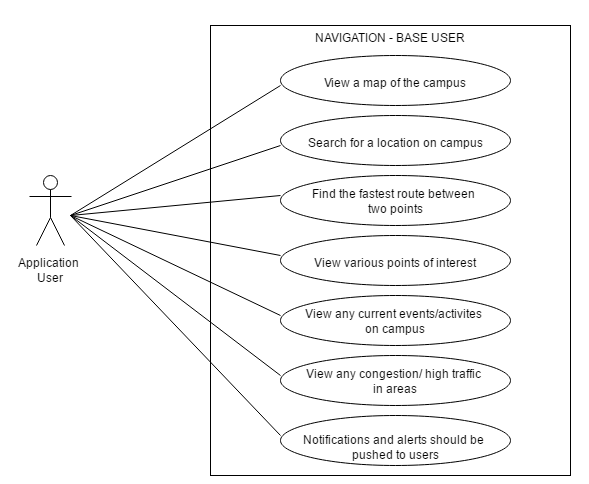
\includegraphics[width=\textwidth]{diagrams/Specific_Requirements/base_user_use_case.png}
\end{figure}
The base user requirements outlines the base/foundation functionality of the system. The inner workings of the system and it's subsystems will be expanded later in the document. Your typical base user will be able to do the following:
\\
\bigskip

\FuncReq
{View the map of campus.}
{The user will be able to view the map through the use of the UI. The map itself will be saved on the system enabling access to it when connected or disconnected. It will contain all locations and venues located on campus itself.}
{Trivial}
{Trivial}
    \\
    \textbf{Actor system interaction model: View the map of campus. }\\
    \begin{tabular}{ | p{6cm} | p{6cm} |}
    \hline
    Actor: Mobile User & System: NavUp \\ \hline
    & 0. The mobile app displays the main menu with the map and map info occupying most of the screen at the default position.\\ \hline
    1. The user scrolls around the map & 2. The app updates the map the map and map info that's in view, pulling information from the remote repository if needed and if possible.\\ \hline
    
    \end{tabular}
\\
\bigskip

\FuncReq
{Search for a location/venue on campus to be displayed on the map.}
{The user needs to be able to search for a location/venue. This will involve a search bar (possible auto-complete functionality) where the user will enter the name of the location/venue. The mobile device will then search through it's database and indicate on the map when the location/venue has been found or display an appropriate prompt when the location/venue is not found.}
{Trivial}
{Trivial}
    \\
    \textbf{Actor system interaction model: Search for a location/venue on campus to be displayed on the map. }\\
    \begin{tabular}{ | p{6cm} | p{6cm} |}
    \hline
    Actor: Mobile User & System: NavUp \\ \hline
    0. The user clicks on the magnification button & 1. The mobile app displays a menu to type in the location and venue.\\ \hline
    2. The user types in the location or venue & 3. Using information from cache and the remote repository, the app tries to perform autocomplete based on what the user is typing.\\ \hline
    4. The user chooses the autocomplete suggestion or types the search term out. & 5. The app generate a list of candidate locations/venues that match its internal cache or the remote repository.\\ \hline
    \end{tabular}
\\
\bigskip


\FuncReq
{Find the fastest route between two points.}%This functional requirement will include finding the start point by gps or by manual input from the user
{
  \begin{enumerate}
    \item The user will be able to set the start point in the following ways:
      \begin{enumerate}
        \item By clicking on the map to indicate the start point or typing the name of the location into the search bar as described in another functional requirement. This should work for both online and offline.
        \item The start point is determined by integrating information from various sensors such as wifi and cellphone tower triangulation, gps, accelerometer and gyroscope. The functionality may work for both online and offline if possible.
      \end{enumerate}

    \item The user will be able to set the end point by tapping on the map to indicate the end point or typing the name of the location into the search bar as described in another functional requirement. This should work for both online and offline.
    \item After setting the start and end point the mobile app must calculate the fastest path between these two points and provide the directions to the user. If the device is offline it must make use of cached data to make an informed choice. If it is online, it must consult the remote repository for the most up to date congestion data.
  \end{enumerate}
  \mbox{}%enumerations cannot be ended with a newline
}
{Trivial}
{Trivial}
    \\
    \textbf{Actor system interaction model:Find the fastest route between two points. }\\
    \begin{tabular}{ | p{6cm} | p{6cm} |}
    \hline
    Actor: Mobile User & System: NavUp \\ \hline
    0. The user clicks on the navigation button & 1. The mobile app displays a menu to type in the starting point and end point.\\ \hline
    2. The user selects the starting point by making a mark on the map or setting it as current location of the mobile device or searching for a place on the map & 3. If the mobile device is online, the remote server sends up to date congestion data to the mobile device. If the mobile device is offline, it uses cached data. In both cases the mobile phone calculate the fastest path using the congestion data, then displays the fastest path to the user.\\ \hline
    \end{tabular}
\\
\bigskip

\FuncReq
{View various points of interest.}
{When selecting a certain building or location the mobile device should display information where applicable for the user to review. When offline the mobile device will use whatever it has in cache, if it is online it may consult the remote repository for the most up to date information.}
{Trivial}
{Trivial}
	\\
    \textbf{Actor system interaction model: View Various Points of Interest. }\\
    \begin{tabular}{ | p{6cm} | p{6cm} |}
    \hline
    Actor: Mobile User & System: NavUp \\ \hline
    & 0. The mobile app displays a map of the campus.\\ \hline
    1. The user selects a destination & 2. The mobile application will display various points of interest along the path to the destination.\\ \hline
    \end{tabular}
\\
\bigskip

\FuncReq
{View any current events or activities happening on campus.}
{The mobile device should display various events and activities happening on campus on the current day as well as upcoming events and activities. When offline it should attempt to display activities and events that have not expired that resides in cache. When online, it should retrieve the most up to date list of events and activities from the remote repository.}
{Trivial}
{Trivial}
	\\
    \textbf{Actor system interaction model: View any current events or activities happening on campus. }\\
    \begin{tabular}{ | p{6cm} | p{6cm} |}
    \hline
    Actor: Mobile User & System: NavUp \\ \hline
    & 0. The mobile app displays a map of the campus.\\ \hline
    1. The user selects a destination & 2. The mobile application will display various activities at venues along the way to the users destination.
    \\ \hline
    \end{tabular}
\\
\bigskip

\FuncReq
{Users should be able to view any congestion/ high traffic in areas.}
{When using the application in a map view of the campus, users should be able to view the amount of pedestrian traffic in surrounding areas. In addition to this any congestion in areas will also be indicated, this could be in the form of pedestrians or any other kind.}
{Trivial}
{Trivial}
\bigskip
	\\
    \textbf{Actor system interaction model: Users should be able to view any congestion/ high traffic in areas.}\\
    \begin{tabular}{ | p{6cm} | p{6cm} |}
    \hline
    Actor: Mobile User & System: NavUp \\ \hline
    & 0. The mobile app displays a map of the campus.\\ \hline
    1. The user selects to view an indication of the pedestrian traffic and congestion on campus & 2. The mobile application will display various points at which there is high congestion and traffic.\\ \hline
    \end{tabular}
\\
\bigskip

\FuncReq
{View the map of campus.}
{The user will be able to view the map through the use of the UI. The map itself will be saved on the system enabling access to it when connected or disconnected. It will contain all locations and venues located on campus itself.}
{Trivial}
{Trivial}
    \\
    \textbf{Actor system interaction model: View the map of campus. }\\
    \begin{tabular}{ | p{6cm} | p{6cm} |}
    \hline
    Actor: Mobile User & System: NavUp \\ \hline
     & 0. The mobile app displays the main menu with the map and map info occupying most of the screen at the default position.\\ \hline
    1. The user scrolls around the map & 2. The app updates the map the map and map info that's in view, pulling information from the remote repository if needed and if possible.\\ \hline
    
    \end{tabular}
\\
\bigskip

\FuncReq
{Emergency notifications and alerts should be pushed to users.}
{The mobile app will receive broadcasts from the remote repository in the event of a emergency. In emergency situations the application could be used to give users directions to assembly places or other appropriate directions.}
{A disaster scenario has taken place and device is connected.}
{Trivial}
    \\
    \textbf{Actor system interaction model: Notifications and alerts should be pushed to users. }\\
    \begin{tabular}{ | p{6cm} | p{6cm} |}
    \hline
    Actor: Mobile User & System: NavUp \\ \hline
    & 0. The remote repository broadcasts an emergency message to connected mobile devices. \\ \hline
    1. The mobile application will display alerts and important messages in the form of notifications on the mobile device. & \\ \hline
    2. The user can click on the notification to view an expanded explanation and description. & 3. The repository may push emergency routes to users if needed.\\ \hline
    
    \end{tabular}
\\
\bigskip

\paragraph{Disabled User requirements}\mbox{}\\
The Disabled User Requirements extends the Base User Requirements. The aim of the disabled navigation is to accommodate disabled users be it students, employees or visitors to successfully use the system.

\FuncReq
{Select voice-assistance.}
{The user can select the voice assistance function so that the mobile application may use voice-commands instead of manually selecting the mobile application's functions.}
{User must be logged in as a disabled user.}
{Interaction between the application and user occur in a verbal manner.}
    \\
    \textbf{Actor system interaction model: Select voice-assistance.}\\
    \begin{tabular}{ | p{6cm} | p{6cm} |}
    \hline
    Actor: Disabled User & System: NavUp \\ \hline
     & 0. The mobile app displays an option to choose a voice command function to communicate with the user.\\ \hline
    1. The user selects to employ the functionality. & 2. The application communicates to the user by use of audible commands as well as a visual representation.\\ \hline
    3. The user may respond in the form of a voice command or by using the touch interface on the mobile device. & \\ \hline
    
    \end{tabular}
\\
\bigskip

\FuncReq
{Color vision deficiency check box.}
{The user is able to adjust the color displayed by the system in the case of a user with color vision deficiency.}
{User must be logged in as a disabled user.}
{Visual aspects of the system are displayed in a format that is visible/audible to the user.}
    \\
    \textbf{Actor system interaction model: Color vision deficiency check box.}\\
    \begin{tabular}{ | p{6cm} | p{6cm} |}
    \hline
    Actor: Disabled User & System: NavUp \\ \hline
     & 0. The mobile app displays an option to choose a contrast in colors that is suitable for the user.\\ \hline
    1. The user selects their preferred view. & 2. The visuals of the application are displayed in the contrast selected by the user.\\ \hline   
    \end{tabular}
\\
\bigskip

\FuncReq
{View the map of campus.}
{This function is the same as in the base user requirements but also accommodates the vision deficiency in terms of the colors used. It will also provide various disabled access points in the form of visual indication on the map or through voice interaction.}
{User must be logged in as a disabled user.}
{Visual aspects of the system are displayed in a format that is visible/audible to the user.}

\FuncReq
{Search for a location/venue on campus to be displayed on the map}
{The user needs to be able to search for a location/venue as stated in the base requirements.The system will display on the map if found or alert the user via voice-command or alert message if not found.}
{User must be logged in as a disabled user.}
{Interaction between the application and user occur in a verbal manner.}

\FuncReq
{Find the fastest route between two points that are wheel chair friendly.}%This functional requirement will include finding the start point by gps or by manual input from the user
{This requirement is the same as the base user requirements but includes the voice-command and also accommodates vision deficiency. The mobile application will navigate a path for the user that is disabled and wheelchair friendly, allowing them to navigate with minimal obstruction.}
{User must be logged in as a disabled user.}
{Interaction between the application and user occur in a verbal manner or a visual manner as determined by the user.}

\FuncReq
{View various points of interest.}
{This requirement is the same as the base user requirements but includes the voice-command and also accommodates vision deficiency.}
{User must be logged in as a disabled user.}
{Interaction between the application and user occur in a verbal manner or a visual manner as determined by the user.}

\FuncReq
{View any current events or activities happening on campus.}
{This requirement is the same as the base user requirements but includes the voice-command and also accommodates vision deficiency.}
{User must be logged in as a disabled user.}
{Interaction between the application and user occur in a verbal manner or a visual manner as determined by the user.}

\FuncReq
{Emergency button.}
{The user can use this special feature to alert the system in the event of an emergency so that nearest wheel chair friendly route to exit point for the disabled user can be displayed.The feature uses the current location of the user to find the fastest wheel chair friendly route.}
{User must be logged in as a disabled user.}
{Emergency personnel are sent to assist the user.}
    \\
    \textbf{Actor system interaction model: Emergency Button}\\
    \begin{tabular}{ | p{6cm} | p{6cm} |}
    \hline
    Actor: Disabled User & System: NavUp \\ \hline
     & 0. The mobile application will display an emergency button or recognise an emergence use-phrase.\\ \hline
    1. The user invokes the use of the emergency button or phrase. & 2. The emergency personnel are notified and are provided with the location of the user.\\ \hline   
    \end{tabular}
\\
\bigskip

\paragraph{Logged-in User requirements}\mbox{}\\
The logged in user will have certain privileges over and above those of the base and guest users. There are two types of logged in users, namely students and lecturers who would log into the system using some form of user-name and password. The typical logged in user will be able to do the following:

\begin{figure}[h] 
  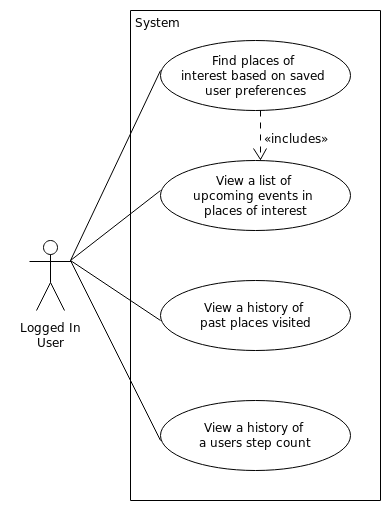
\includegraphics[width=0.5\textwidth]{diagrams/Specific_Requirements/Loggedin_User_Case_Diagram.png}
\end{figure}

\mbox{}\\
\bigskip

\FuncReq
{Find places of interest based on saved user preferences.}
{The users will be given the option to populate a list of preferred preferences and places of interest. The system will then generate and display a list, when needed, of the  places of interest and various events that are happening currently. This list that is provided to the user is unique and tailored to them.}
{User needs to be logged in.}
{Trivial}
\\
    \textbf{Actor system interaction model: Find places of interest based on saved user preferences. }\\
    \begin{tabular}{ | p{6cm} | p{6cm} |}
    \hline
    Actor: Logged In User & System: NavUp \\ \hline
    & 0. The system gathers all information on the logged in user.\\ \hline
    1. The user opens prefrences on points of interests. & 2. The mobile application will display various points of interest.\\ \hline
    3. The user selects various prefrences. & 4. The system updates the user's data on prefrences. \\ \hline
    & 5. The mobile application generates and displays a list of places of interest. \\ \hline
    \end{tabular}
\\
\bigskip

\FuncReq
{View a list of upcoming events in places of interest.}
{Using the saved list of preferences and places of interest that the user has provided, the system will automatically generate a list of the upcoming events that are taking place at these places and the user will be able to view them in a time-line manner and set reminders for these events.}
{User needs to be logged in.}
{Trivial}
\\
    \textbf{Actor system interaction model: View a list of upcoming events in places of interest. }\\
    \begin{tabular}{ | p{6cm} | p{6cm} |}
    \hline
    Actor: Logged In User & System: NavUp \\ \hline
    0. The user opens upcoming events and activities. & 1. The mobile application will display various upcoming events and activities.\\ \hline
    3. The user sets reminders to preferred events and activities. & 4. The system saves the reminders in the database. \\ \hline
    & 5. The mobile application notifies the user when an event is happening at appropriate times. \\ \hline
    \end{tabular}
\\
\bigskip

\FuncReq
{View a history of past places visited.}
{Users will be able to view a history of the past events that they have attended. This will include the type of event that took place and the location that the event was at.}
{User needs to be logged in.}
{Trivial}
\\
    \textbf{AView a history of past places visited. }\\
    \begin{tabular}{ | p{6cm} | p{6cm} |}
    \hline
    Actor: Logged In User & System: NavUp \\ \hline
    0. The user opens their history. & 1. The mobile application will display various locations and events the user has attended/visited.\\ \hline
    \end{tabular}
\\
\bigskip

\FuncReq
{View a history of a users step count.}
{The system will will track and record the step-count of each user, this history will be viewable by the user according to the time-line that the user will be able to specify.}
{User needs to be logged in.}
{Trivial}
\\
    \textbf{Actor system interaction model: View a history of a users step count. }\\
    \begin{tabular}{ | p{6cm} | p{6cm} |}
    \hline
    Actor: Logged In User & System: NavUp \\ \hline
    0. The user opens their profile/user information. & 1. The mobile application will display statistics of the user's step count.\\ \hline
    3. The user adjusts the timeline to view the amount of steps taken. & 4. The mobile application updates the information accordingly. \\ \hline
    \end{tabular}
\\
\bigskip

\paragraph{Guest User requirements}\mbox{}\\
In regards to the Guest Users, they will have the same requirements of a Base User (See Base User Requirements). They won't have an associative ID linking them to the database seeing as they will not be logged in. As soon as they do so they will be seen as a Logged In User. The only possible added functionality will be catering to people who don't visit campus often. See below mentioned for expanded requirements:

\FuncReq
{A better view of points of interest on the map.}
{A guest user will most likely be someone visiting campus. It will thus be beneficial to the user if the points of interest are more visible to them. This will allow them to easily find any usefull information they might need. This can be done by highlighting or setting points on the map itself for the user to select and read further information on that point.}
{Trivial}
{Trivial}
\\
\textbf{Actor system interaction model: A better view of points of interest on the map.}\\
\begin{tabular}{ | p{6cm} | p{6cm} |}
\hline
Actor: Mobile Guest User & System: NavUp \\ \hline
& 0. The mobile app displays a map of the campus.\\ \hline
1. The user selects a destination & 2. The mobile application will display in a more visual way various points of interest along the path to the destination.\\ \hline
\end{tabular}
\\
\bigskip
\\    
\textbf{Actor system interaction model: A better view of points of interest on the map. }\\
\begin{tabular}{ | p{6cm} | p{6cm} |}
\hline
Actor: Mobile Guest User & System: NavUp \\ \hline
& 0. The mobile app displays a map of the campus.\\ \hline
1. The user selects a location on the map & 2. The mobile application will display in a more visual way various points of interest in the surrounding areas.\\ \hline
\end{tabular}
\\
\bigskip

\FuncReq
{A better view of activities/events happening on campus.}
{Campus plays host to various events and activities like Business days or even music orchestras. This means that campus will have a number of guests unfamiliar with the layout of campus or the location of these activities/events. The guest user needs to be able to view the activities/events in a more visible way. This will allow them to navigate to their destination and/or read more information on it. This can also be displayed on the map or even on a sub-menu for ease of access.}
{Trivial}
{Trivial}
\\
\textbf{Actor system interaction model: A better view of activities/events happening on campus.}\\
\begin{tabular}{ | p{6cm} | p{6cm} |}
\hline
Actor: Mobile Guest User & System: NavUp \\ \hline
& 0. The mobile app displays a map of the campus.\\ \hline
1. The user selects a destination & 2. The mobile application will display in a more visual way various events and activities along the path to the destination.\\ \hline
\end{tabular}
\\
\bigskip
\\    
\textbf{Actor system interaction model: A better view of activities/events happening on campus. }\\
\begin{tabular}{ | p{6cm} | p{6cm} |}
\hline
Actor: Mobile Guest User & System: NavUp \\ \hline
& 0. The mobile app displays a map of the campus.\\ \hline
1. The user selects a location on the map & 2. The mobile application will display in a more visual way various events and activities happening in the surrounding areas.\\ \hline
\end{tabular}
\\
\bigskip



\subsubsection{Agent Requirements}
\paragraph{Agent User Requirements}\mbox{}\\
The agent is a metaphor for the system itself in a higher privilege right, such that it will have access to all the users' information and be able to analyse this, after which meaningful data will be generated from there and be used to form the real-time notifications that will be pushed to other users. The agent will be able to do the following:
\\
\bigskip

\FuncReq
{Analyse and integrate the information sent from user devices}
{The agent will have access to different forms of data that the users will continuously send to it and the agent organises this data so that meaningful information can be extrapolated and used. This data will be in the form of location coordinates, stagnant users, step counters,user preferences and places of interest time taken on a specific route and possibly more. This data will then be analysed by the agent and real-time feedback will be given back to the users in terms of fastest routes, traffic congestion, places they may be interested in, nearby events, surveillance information and possibly more.}
{TODO}
{TODO}
    \\
    \textbf{Actor system interaction model: Analyse and integrate information sent from user devices }\\
    \begin{tabular}{ | p{6cm} | p{6cm} |}
    \hline
    Actor: Mobile User & System: NavUp Agent\\ \hline
     0. The mobile user opens the application and has a view of the UP campus map & 1. The mobile application will display and indicate areas of high congestion, places of interest.\\ \hline
    
    \end{tabular}
\\
\bigskip


\FuncReq
{Privilege management and authentication}
{The agent will be able to distinguish between the different types of users and convey the relevant information to them as well as differentiate the type of access rights that each type of user has on the data, for example mobile users will only have read access to congestion data, agents will have read and write data and administrators will have read and write access on the data.}
{TODO}
{TODO}
One of the concerns raised by the developing team was the issue of the life time of the system/mobile application. Students might not see the benifit of the mobile apllication seeing that the majority of students know the layout of campus and where venues are located. The client mentioned incentive in the form of a Goal and Reward System. The client did not expand on this issue so this might be subject to change. Here are a few requirements if such a system was implemented in NavUP:

\FuncReq
{Track the user's steps or distance walked.}
{The mobile application will have to keep track of the users steps or measure the distance they have walked. This data will be saved and used when tracking the goals and achievements of the user. It will also be visible to the user for them to see how much/far they have walked.}
{The user needs to be logged in.
The user needs to maintain some form of connection.}
{TODO}
\\
\textbf{Actor system interaction model: Track the user's steps or distance walked.}\\
\begin{tabular}{ | p{6cm} | p{6cm} |}
\hline
Actor: Mobile User & System: NavUp \\ \hline
& 0. The mobile application will keep track of the users steps taken and/or distance traveled.\\ \hline
& 1. The mobile application saves this data and the system stores it on the database.\\ \hline
\end{tabular}
\\
\bigskip

\FuncReq
{Display the various fun run routes on campus.}
{Campus has varius fun run routes marked by painted animal footprints. These footprints have in time faded away, therefore it will be benefitial to display these routes to the user when they want to reach a certain goal or even just have a jog for exercise. This can be displayed on the map as a navigational route.}
{The user needs to be logged in.
The user needs to maintain some form of connection.}
{TODO}
\\
\textbf{Actor system interaction model: Display the various fun run routes on campus.}\\
\begin{tabular}{ | p{6cm} | p{6cm} |}
\hline
Actor: Mobile User & System: NavUp \\ \hline
0. The user selects the fun run routes. & 1. The mobile application displays the various fun run routes on the map.\\ \hline
2. The user chooses a fun run route to complete. & 3. The mobile application starts the navigation of that route.\\ \hline
& 4. The mobile application tracks the user's progress until the route is finished.\\ \hline
\end{tabular}
\\
\bigskip

\FuncReq
{Set goals for the user to finish.}
{The client has not expanded on this section, therefore there can only be assumed that the mobile app will have certain goals/achievements listed. This will most likely be in the form of a certain distance walked or a number of steps taken. These goals will have to be set by the administrators and will have various levels of completion, each level awarding a prize to the user.}
{The user needs to be logged in.
The user needs to maintain some form of connection.}
{TODO}
\\
\textbf{Actor system interaction model: Set goals for the user to finish.}\\
\begin{tabular}{ | p{6cm} | p{6cm} |}
\hline
Actor: Mobile User & System: NavUp \\ \hline
0. The user selects the goals on the mobile application. & 1. The mobile application displays the various goals for the user to complete.\\ \hline
2. The user selects a goal to complete. &\\ \hline
\end{tabular}
\\
\bigskip

\FuncReq
{Notify the user when they have reached/completed a goal.}
{The mobile app will have to notify the user when they have reached a certain goal or even a user's personal goal. This will allow the user to move to the next goal. This can be done via push notifications. The goals can also be tracked by the user to see how far they are from completing it.}
{The user needs to be logged in.
The user needs to maintain some form of connection.}
{TODO}
\\
\textbf{Actor system interaction model: Notify the user when they have reached/completed a goal.}\\
\begin{tabular}{ | p{6cm} | p{6cm} |}
\hline
Actor: Mobile User & System: NavUp \\ \hline
& 0. The mobile application tracks the user's progress on certain goals.\\ \hline
& 1. The mobile application notifies the user when a goal has been completed.\\ \hline
2. The user selects the next goal to complete & 3. The mobile application starts to track the progress of the next goal.\\ \hline
\end{tabular}
\\
\bigskip

\FuncReq
{Display the user's statistics for review.}
{The mobile app will need a statistics section where the overall progress and steps taken/distance traveled will be recorded and displayed. This may include maximum distance walked in a day to average step count depending on the clients final wishes on this section.}
{The user needs to be logged in.
The user needs to maintain some form of connection.}
{TODO}
\\
\textbf{Actor system interaction model: Display the user's statistics for review. }\\
\begin{tabular}{ | p{6cm} | p{6cm} |}
\hline
Actor: Logged In User & System: NavUp \\ \hline
0. The user opens their profile/user information. & 1. The mobile application will display statistics of the user's step count.\\ \hline
2. The user adjusts the timeline to view the amount of steps taken. & 3. The mobile application updates the information accordingly. \\ \hline
\end{tabular}
\\
\bigskip

\FuncReq
{Notify the user when they have been awarded a prize.}
{The mobile app will also need to notify the user when they have been awarded a prize. These prizes will be the responsibility of the client and it is up to them to set when such a prize is rewarded. The notification will then display a message of what the user has won.}
{The user needs to be logged in.
The user needs to maintain some form of connection.}
{TODO}
\\
\textbf{Actor system interaction model: Notify the user when they have been awarded a prize.}\\
\begin{tabular}{ | p{6cm} | p{6cm} |}
\hline
Actor: Logged In User & System: NavUp \\ \hline
& 0. The mobile application will track the progress of a prize.\\ \hline
& 1. The mobile application will notify the user when they have been rewarded a prize.\\ \hline
& 2. The mobile application will track the progress of the next prize.\\ \hline
\end{tabular}
\\
\bigskip

\FuncReq
{Display information/guide of how users can collect their prizes.}
{The client will have to provide the information needed to collect a prize and where to do so. This information will then be displayed to the user along with contact details if anything is uncertain. Again this is up to the client and how they want to implement this section, for now only assumptions can be made.}
{The user needs to be logged in.
The user needs to maintain some form of connection.}
{TODO}
\\
\textbf{Actor system interaction model: Display information/guide of how users can collect their prizes.}\\
\begin{tabular}{ | p{6cm} | p{6cm} |}
\hline
Actor: Logged In User & System: NavUp \\ \hline
& 0. When a prize has been awarded the mobile application will display information on how to collect the prize\\ \hline
& 1. The mobile application will also display contact details to the user for any queries.\\ \hline
2. The user follows these instructions to claim their prize. &\\ \hline
\end{tabular}
\\
\bigskip
\subsubsection{Goals and Prizes}
\paragraph{Goals and Prizes}\mbox{}\\
One of the concerns raised by the developing team was the issue of the life time of the system/mobile application. Students might not see the benifit of the mobile apllication seeing that the majority of students know the layout of campus and where venues are located. The client mentioned incentive in the form of a Goal and Reward System. The client did not expand on this issue so this might be subject to change. Here are a few requirements if such a system was implemented in NavUP:

\FuncReq
{Track the user's steps or distance walked.}
{The mobile application will have to keep track of the users steps or measure the distance they have walked. This data will be saved and used when tracking the goals and achievements of the user. It will also be visible to the user for them to see how much/far they have walked.}
{The user needs to be logged in.
The user needs to maintain some form of connection.}
{TODO}
\\
\textbf{Actor system interaction model: Track the user's steps or distance walked.}\\
\begin{tabular}{ | p{6cm} | p{6cm} |}
\hline
Actor: Mobile User & System: NavUp \\ \hline
& 0. The mobile application will keep track of the users steps taken and/or distance traveled.\\ \hline
& 1. The mobile application saves this data and the system stores it on the database.\\ \hline
\end{tabular}
\\
\bigskip

\FuncReq
{Display the various fun run routes on campus.}
{Campus has varius fun run routes marked by painted animal footprints. These footprints have in time faded away, therefore it will be benefitial to display these routes to the user when they want to reach a certain goal or even just have a jog for exercise. This can be displayed on the map as a navigational route.}
{The user needs to be logged in.
The user needs to maintain some form of connection.}
{TODO}
\\
\textbf{Actor system interaction model: Display the various fun run routes on campus.}\\
\begin{tabular}{ | p{6cm} | p{6cm} |}
\hline
Actor: Mobile User & System: NavUp \\ \hline
0. The user selects the fun run routes. & 1. The mobile application displays the various fun run routes on the map.\\ \hline
2. The user chooses a fun run route to complete. & 3. The mobile application starts the navigation of that route.\\ \hline
& 4. The mobile application tracks the user's progress until the route is finished.\\ \hline
\end{tabular}
\\
\bigskip

\FuncReq
{Set goals for the user to finish.}
{The client has not expanded on this section, therefore there can only be assumed that the mobile app will have certain goals/achievements listed. This will most likely be in the form of a certain distance walked or a number of steps taken. These goals will have to be set by the administrators and will have various levels of completion, each level awarding a prize to the user.}
{The user needs to be logged in.
The user needs to maintain some form of connection.}
{TODO}
\\
\textbf{Actor system interaction model: Set goals for the user to finish.}\\
\begin{tabular}{ | p{6cm} | p{6cm} |}
\hline
Actor: Mobile User & System: NavUp \\ \hline
0. The user selects the goals on the mobile application. & 1. The mobile application displays the various goals for the user to complete.\\ \hline
2. The user selects a goal to complete. &\\ \hline
\end{tabular}
\\
\bigskip

\FuncReq
{Notify the user when they have reached/completed a goal.}
{The mobile app will have to notify the user when they have reached a certain goal or even a user's personal goal. This will allow the user to move to the next goal. This can be done via push notifications. The goals can also be tracked by the user to see how far they are from completing it.}
{The user needs to be logged in.
The user needs to maintain some form of connection.}
{TODO}
\\
\textbf{Actor system interaction model: Notify the user when they have reached/completed a goal.}\\
\begin{tabular}{ | p{6cm} | p{6cm} |}
\hline
Actor: Mobile User & System: NavUp \\ \hline
& 0. The mobile application tracks the user's progress on certain goals.\\ \hline
& 1. The mobile application notifies the user when a goal has been completed.\\ \hline
2. The user selects the next goal to complete & 3. The mobile application starts to track the progress of the next goal.\\ \hline
\end{tabular}
\\
\bigskip

\FuncReq
{Display the user's statistics for review.}
{The mobile app will need a statistics section where the overall progress and steps taken/distance traveled will be recorded and displayed. This may include maximum distance walked in a day to average step count depending on the clients final wishes on this section.}
{The user needs to be logged in.
The user needs to maintain some form of connection.}
{TODO}
\\
\textbf{Actor system interaction model: Display the user's statistics for review. }\\
\begin{tabular}{ | p{6cm} | p{6cm} |}
\hline
Actor: Logged In User & System: NavUp \\ \hline
0. The user opens their profile/user information. & 1. The mobile application will display statistics of the user's step count.\\ \hline
2. The user adjusts the timeline to view the amount of steps taken. & 3. The mobile application updates the information accordingly. \\ \hline
\end{tabular}
\\
\bigskip

\FuncReq
{Notify the user when they have been awarded a prize.}
{The mobile app will also need to notify the user when they have been awarded a prize. These prizes will be the responsibility of the client and it is up to them to set when such a prize is rewarded. The notification will then display a message of what the user has won.}
{The user needs to be logged in.
The user needs to maintain some form of connection.}
{TODO}
\\
\textbf{Actor system interaction model: Notify the user when they have been awarded a prize.}\\
\begin{tabular}{ | p{6cm} | p{6cm} |}
\hline
Actor: Logged In User & System: NavUp \\ \hline
& 0. The mobile application will track the progress of a prize.\\ \hline
& 1. The mobile application will notify the user when they have been rewarded a prize.\\ \hline
& 2. The mobile application will track the progress of the next prize.\\ \hline
\end{tabular}
\\
\bigskip

\FuncReq
{Display information/guide of how users can collect their prizes.}
{The client will have to provide the information needed to collect a prize and where to do so. This information will then be displayed to the user along with contact details if anything is uncertain. Again this is up to the client and how they want to implement this section, for now only assumptions can be made.}
{The user needs to be logged in.
The user needs to maintain some form of connection.}
{TODO}
\\
\textbf{Actor system interaction model: Display information/guide of how users can collect their prizes.}\\
\begin{tabular}{ | p{6cm} | p{6cm} |}
\hline
Actor: Logged In User & System: NavUp \\ \hline
& 0. When a prize has been awarded the mobile application will display information on how to collect the prize\\ \hline
& 1. The mobile application will also display contact details to the user for any queries.\\ \hline
2. The user follows these instructions to claim their prize. &\\ \hline
\end{tabular}
\\
\bigskip
\paragraph{Goals Web UI}\mbox{}\\
\begin{figure} 
  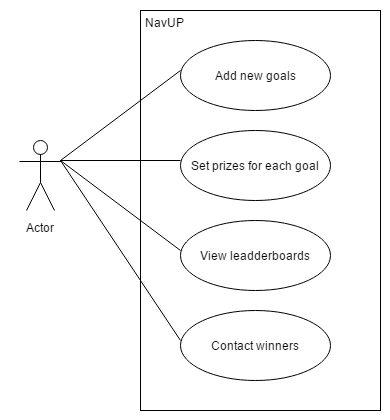
\includegraphics[width=\textwidth]{diagrams/Specific_Requirements/Goals_WebUI_Actor_Syetem_Interaction.png}
\end{figure}

The Web User Interface will be used by system administrators to manage the system, as such the Web UI for goals and activities will be managed on this interface.
\\
\bigskip
\FuncReq
{CRUD goals and activities.}
{The system shall provide an interface for an admin user to add and create goals for the users to aim to achieve. The admin must be able to set what the requirements to reach the goals are, and the time frame allocated for achieving these goals, such as daily or weekly. The admin will also be able to see which users have met the goals that have been set. This data should be able  to be sorted by time taken to reach the goal or by who achieved the highest score in order to decide on who can win a prize.}
{The admin user must be authorised in order to make changes to the system.}
{Trivial}

\FuncReq
{CRUD prizes.}
{The system shall provide a way to add prizes that may be won by users as an incentive for completing goals. Each goal will be able to have a prize associated with it so that the user may see what they are eligible to win for completing the goal. Harder goals to achieve can then have better prizes associated with them to add to the incentive. The system shall display users who have achieved a goal and are eligible to win a prize. The choosing of a winner for a goal is at the discretion of the admin. Contact options for user who have completed the goal will be available to the admin in order to inform them of their prize.}
{User must be authorised}
{Trivial}

